% !TEX TS-program = pdflatexmk
\documentclass[11pt]{article}
\usepackage[margin=.75in]{geometry} 
\usepackage[parfill]{parskip}
\usepackage{graphicx,booktabs}
%SetFonts
% libertine text and newtxmath
\usepackage{newpxtext}
\usepackage[TS1,T1]{fontenc}
\usepackage{textcomp}
\usepackage[scaled=.85]{beramono} 
\usepackage{newpxmath}
\usepackage[npx]{superiors}
\makeatletter
\def\libertine@figurestyle{OsF}
\makeatother
%\def\libertine{\fontfamily{fxlj}\selectfont}
%SetFonts
%\usepackage[supstfm=libertinesups,%
%  supscaled=1.2,%
%  raised=-.13em,
%  supscolor=red]{superiors}
\title{Superiors}
\author{Michael Sharpe}
\date{\today}  % Activate to display a given date or no date

\begin{document}
\maketitle
\section*{Briefly}
Superior letters, figures and symbols are most commonly used as footnote markers but are occasionally used to imitate eighteenth century writing abbreviations such as M\textsu{me}. Footnote markers in \LaTeX\ are superscripted versions of characters governed by the regimes in which they appear---title, minipage and body. Normally, those generated in the body of a document are successive integers starting at 1, while those in a minipage are italic letters beginning at \emph{a} and those in the document title use symbols like \textasteriskcentered, \textdagger, etc. 

The default behavior of footnote markers in \LaTeX\ is to typeset the marker as if it were a mathematical superscript. In most cases, this means the size is about 70\% of the normal lining figure and the top is a bit above the tops of capital letters. They appear rather slight compared to normal text.


As an alternative, one may use superior figures---small figures, usually 50\% to 70\% of the height of lining figures, like \textsu{1234567890}. Commonly, they are designed so that the tops of the numbers are aligned with the tops of the capital letters in the font, though sometimes a little higher, corresponding to the ascender height. 

This package, now updated to version~2, expands on the macros of version~1 and works with {\tt lualatex}, {\tt xelatex} and legacy {\tt [pdf]latex}, and with document classes defined in {\tt latex.ltx}, the AMS classes and the KOMA classes. It also cooperates with {\tt realscripts}, which it calls under both {\tt lualatex} and {\tt xelatex}, leaving most of its macro definitions unchanged except for \verb|\@makefnmark|. Unlike version~1, which based the replacement superiors by means of a specified {\tt tfm} file, with version~2  you must specify  either a  latex font family name or an {\tt otf} filename ({\tt lualatex} and {\tt xelatex} only.) The macro that does the work is \verb|\textfnscript|.

\section*{Some Details}
PostScript fonts have for a long time mostly contained just a small subset $\{1,2,3\}$ of the possible superior digits, and most OpenType fonts in the Adobe portfolio, other than the most popular and the most recent, contain the same small subset. Moreover, the \textsf{TS1} encoding includes slots for only those three superior figures. Even the first version of the STIX collection contains just the basic three superior figures.


It is now not uncommon to find Opentype fonts with four vertical levels of small figures. Two of these, numerators and denominators, are supposed to be used only for text fractions, and most commonly the baseline of a denominator is the same as the text baseline, while the top of the numerators is either the height of a lining figure or the cap-height. The other two levels are superiors and either scientific inferiors or  subscripts. (The corresponding opentype lookups are {\tt numr}, {\tt dnom}, {\tt sups}, {\tt sinf} and {\tt subs}.) Most commonly, these figures all have the same size, but is becoming more common for {\tt sups}, {\tt subs} and {\tt sinf} to be about 20\% larger than {\tt numr} and {\tt dnom}. It is also now more common for {\tt sups} to contain a full set of Roman letters and a good selection of text punctuation and symbols. 

This package allows you to substitute a set of superiors  from one font family into a font family that either lacks superiors or has an inadequate set of superiors. Unlike version~1 of this package, version~2 can work with all LaTeX engines and works to some extent with KOMA classes. The methods amount to a variant of Will Robertson's {\tt realscripts} package that isolates the use of {\tt fontspec} to the unicode latex case.

Speaking in general terms, this package does the following:
\begin{itemize}
\item You provide through options to {\tt superiors} the information about the font which will provide the substitutions. 
\item The information may be a latex font family, an otf font or an abbreviation understood by the package from which to draw the superior glyphs. There are three different option types to convey the source for the substitute superiors:
\begin{itemize}
\item
{\tt supsfam=...} may be used to specify the latex font family to be used to render the substitute superiors. If specified, this overrides option choices using {\tt supsotf} or an abbreviated family name. E.g., to substitute superiors from the {\tt ETbb} font:
\begin{verbatim}
\usepackage[supsfam=ETbb-Sup]{superiors}
\end{verbatim}

\item
{\tt supsotf=...} may be used to specify the {\tt otf} to be used to render the substitute superiors. If specified, this overrides option choices using an abbreviated family name. (Ignored except by {\tt lualatex} and {\tt xelatex}.) E.g., to substitute superiors from the {\tt XCharter} otf font:
\begin{verbatim}
\usepackage[supsotf=XCharter-Roman.otf]{superiors}
\end{verbatim}

\item
An abbreviated family name may be used to specify the family/otf to be used to render the substitute superiors. The possible abbreviation options are:
\begin{center}
  \begin{tabular}{@{} lll @{}}
    \toprule
    LaTeX Family Name & Otf Name & Abbreviations \\
    \midrule
    ntxsups & TeXGyreTermesX-Regular.otf & newtx, newtxtext, ntx, ztm \\
    zplsups & TeXGyrePagellaX-Regular.otf & newpx, newpxtext, npx, zpl \\
    LibertinusSerif-Sup & LibertinusSerif-Regular.otf & lbtn, libertine, libertinus \\
    Cochineal-Sup & Cochineal-Roman.otf & coch, cochineal, Cochineal \\
    SticksTooText-Sup & STIXTwoText-Regular.otf & stix2, stickstoo, stickstootext, SticksToo \\
    ETbb--Sup & ETbb-Regular.otf & etbb, ETbb \\
    fbb-Sup & fbb-Regular.otf & fbb \\
    Erewhon-Sup & Erewhon-Regular.otf & erewhon, Erewhon\\
    XCharter-Sup & XCharter-Roman.otf & xch, xcharter, XCharter \\
    BaskervilleF-Sup & BaskervilleF-Regular.otf & baskervillef, Baskerville\\
    Baskervaldx-Sup & Baskervaldx-Regular.otf & baskervaldx, Baskervaldx \\
    zgm1 & • & zgm, garamondx \\
    scholax-Sups & TeXGyreScholaX-Regular.otf & scholax \\
    EBGaramond-Sup & EBGaramond-Regular.otf & ebg, ebgaramond, EBGaramond \\
    \bottomrule
  \end{tabular}
\end{center}
\end{itemize}
\end{itemize}

\textsc{Examples:}
\begin{itemize}
\item
\begin{verbatim}
\usepackage[lbtn, supsfam=Cochineal-Sup]{superiors}
\end{verbatim}
would ignore the {\tt lbtn} because {\tt supsfam=} takes precedence, and similarly with
\begin{verbatim}
\usepackage[lbtn, supsotf=Cochineal-Roman.otf]{superiors}
\end{verbatim}
In both cases, {\tt Cochineal-Roman} superiors would made available to replace the original superiors. Under {\tt lualatex} or {\tt xelatex}, the lines above would be equivalent to
\begin{verbatim}
\usepackage[supsotf=Cochineal-Roman.otf]{superiors}
\end{verbatim}
and under legacy {\tt latex}, to
\begin{verbatim}
\usepackage[supsfam=Cochineal-Sup]{superiors}
\end{verbatim}
\end{itemize}
\textsc{Notes:}
\begin{itemize}
\item
If no source is specified for the replacement superiors, {\tt ntxsups} will be used.
\item
The {\tt superiors} package should be loaded after other font package. 
\item Unless using a legacy latex, {\tt realscripts} will be loaded by {\tt superiors}, if need be.
\item With both {\tt lualatex} and {\tt xelatex}, you may specify a legacy font family for superiors.
\end{itemize}
%\item
%\[Re\]define \verb|\sustyle| and \verb|\textsu| so they lead to the sups family that will be substituted. (The first is a font switch and the second is a macro which applies the font switch to its argument.)
%\end{itemize}
\section*{Other {\tt options}}
 The package also allows you to scale the size of the imported superiors  and to specify an amount by which to raise them. You may also specify a spacing to apply before and after the footnote marker and set a color.
 \begin{itemize}
\item
 {\tt supscale} (or {\tt supscaled}) controls the scale factor applied to superiors. 
 \item
 {\tt supsraised} (or {\tt raised}) controls the amount to raise the superiors. It should have a unit that responds to the overall scaling of the document text, like {\tt em} or {\tt ex}.
\item
{\tt supsLspaced} and {\tt supsRspaced} govern the amount of kerning to be inserted to the Left and Right. (Default value for both is {\tt .04em}.) Option {\tt supspaced} sets its argument to both.
\item
 {\tt supscolor} controls the color applied to superiors. (Default value is {\tt black}.) You may use any color specification understood by the {\tt xcolor} package.
\item
{\tt notitlepatch} causes the \verb|\maketitle| macro, which specifies among other things how footnotes and \verb|\thanks| operate within title, to not be patched to behave like body footnotes. The effect is to not use the superiors modifications within titles. This can be useful if your substitute superiors lack \verb|\textasteriskcentered|, \verb|\textdagger|, etc.
\end{itemize}

\section*{Some Background}
Modern versions of {\tt latex.ltx} define the basic macros for subscripts and superscripts making use of the mathematical superscripts and subscript constructions that involve shrinking fullsize letters, figures and symbols to \verb|\scriptstyle|. The control sequences of importance to superscripts are:
\begin{itemize}
\item
\verb|\@textsuperscript#1| switches to math mode, shrinks \verb|#1| and puts it in an \verb|\mbox| which is rendered as a math superscript.
\item 
\verb|\textsuperscript#1| is a robust macro which applies \verb|\@textsuperscript| to \verb|#1|.
\item 
\verb|\@makefnmark| makes an \verb|\hbox| containing  \verb|\@thefnmark|, the actual character to show as the marker for the footnote, acted upon by \verb|\@textsuperscript|. 
\end{itemize}
The {\tt realscripts} package, which requires {\tt lualatex} or {\tt xelatex}, defines new macros \verb|\fakesuperscript| (essentially, the latex \verb|\textsuperscript|) and \verb|\realsuperscript| (makes use of the superiors in an Opentype font, if available) and then redefines \verb|\textsuperscript| to use \verb|\realsuperscript|, if possible. Then \verb|\@makefnmark| is redefined to make use of \verb|\textsuperscript| while paying attention to whether a KOMA class is active. So, to summarize, in {\tt realscripts}, assuming the {\tt opentype} font is properly set up with superiors:
\begin{itemize}
\item
\verb|\realsuperscript#1| is defined to use those superiors.
\item
\verb|\textsuperscript#1| is redefined to \verb|\realsuperscript#1|.
\item
\verb|\@makefnmark| is redefined to use \verb|\textsuperscript#1| instead of \verb|\@textsuperscript#1|.
\end{itemize}

Part of what happens in {\tt superiors.sty} is making similar code that works in legacy latex and which adds for all latex engines the additional features (scaling, raising, spacing and coloring) that do not appear in {\tt realscripts.})

Meanwhile, there is a separate strand that affects only footnotes and \verb|\thanks| that occur during the processing of \verb|\maketitle|. (This macro is not part of {\tt latex}---it is defined in the document class file, e.g., {\tt article.cls}.) This is where footnote markers other than figures may need to be generated. This package adds patches to the code in \verb|\maketitle| that adds the same feature to footnotes and \verb|\thanks| in that setting.

\textsc{Important Notes:}
\begin{itemize}
\item
{\tt superiors} defines \verb|\realsuperscript| in legacy latex processing and extends \verb|\textsuperscript| to cover all latex engines, not changing the {\tt realscripts} definition where it applies. 
\item 
{\tt superiors} defines a new macro \verb|\textSuperscript| that adds the features mentioned above on top of \verb|\textsuperscript|. This is the basis for a redefinition of \verb|\@makefnmark| that uses real superior glyphs, where possible.
\item
Many font packages, especially those generated by {\tt autoinst}, define macros \verb|\sustyle| (or \verb|\sufigures|) and \verb|\textsu| that may be used to specify superiors. The first two are simple text switches and the latter is a macro that applies the switch to its argument. I don't think there is any official latex position about these names. These macros are not affected by the options mentioned above, and nor are \verb|\textsuperscript| and \verb|\realsuperscript|. The macro that does respond to the package options \verb|\textfnscript|, which is used for footnote markers. E.g., \verb|\textfnscript{abc}| produces \textfnscript{abc} provided your superiors font has those glyphs.

\end{itemize}

\section*{Sample Invocations}

\begin{itemize}
\item Times-like, no rescaling or raising, but with $.03${\tt em} space before and after footnote markers:
\begin{verbatim}
\usepackage[supspaced=.03em]{superiors} % default value is .04em
\end{verbatim}
\item Add colored {\tt newtx} superiors to {\tt newtx}, no rescaling or raising:
\begin{verbatim}
\usepackage{newtx}
\usepackage[supscolor=red!70!black]{superiors} \end{verbatim}
\item Libertine superiors scaled up by 20\%, then lowered:
\begin{verbatim}
\usepackage{libertine}
\usepackage[lbtn,%
  supscaled=1.2,%
  raised=-.13em]% match ascender height of libertine
{superiors}
\end{verbatim}
%\item Use MinionPro\footnote{Assumes you have installed MinionPro according to the directions in the \textsf{minion2newtx} package.}
% superiors at default size, lowered a bit:
%\begin{verbatim}
%\usepackage[supstfm=T1-Minion2Pro-Regular-sups-kern-liga,%
%  raised=-.05em]%
%{superiors}
%\end{verbatim}
\end{itemize}

%It is best to specify a relative unit for the {\tt raised} and {\tt supspaced} parameters so that they change with the font size. (Recall that for a $10${\tt pt} font, {\tt 1em} is usually {\tt 10pt}, but the actual size of {\tt 1em} is defined relative to font size.)

The following example compares libertine with its default footnote markers against libertine with the superiors package as described in the example above:

\[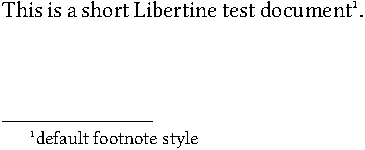
\includegraphics{libfoot0-crop} \qquad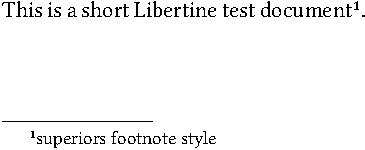
\includegraphics{libfoot1-crop}\]

%There is another parameter named {\tt scaled} that should be used only if you loaded your text font with a scale parameter different from $1.0$, and in this case, you should use the same scale parameter. For example:
%\begin{verbatim}
%\usepackage[lining,scaled=1.05]{bembo}
%\usepackage[scaled=1.05,%
%  lbtn,% libertine
%  supscaled=1.2,%
%  raised=-.13em]%
%{superiors}
%\end{verbatim}
\section*{Issues with superiors}
%If a number of figure styles are available, many packages make use of \textsf{nfssext} (or its further extension \textsf{nfssext-cfr}) to access those special forms. For superior figures, two macros are defined by \textsf{nfssext}: 
%\verb|\sustyle| and \verb|\textsu|, the first of which changes the text font to a font with superior figures (and is usually called with action confined to a group), while the second is a macro called like \verb|\textsu{123}| which applies \verb|\sustyle| to just its argument. In packages generated by {\tt otfinst} and {\tt autoinst}, if superior figures are available (even if only three of them), \verb|\sustyle| and \verb|\textsu| are defined and refer to the superior figures. Moreover, \verb|otfinst| redefines \verb|\@makefnmark|:
%\begin{verbatim}
%\def\@makefnmark{\hbox{\sustyle\@thefnmark}}
%\end{verbatim}
%so that it uses figures in \verb|\sustyle|. 
You may run into problems with older fonts having just three superior figures \textsu{123}
because footnote marker figures greater than three will render using normal size figures. For example, in Stempel Garamond, where there are only three superior figures available, the first graphic shows the default footnote markers, the second shows the document processed with libertine footnote markers using 
\begin{verbatim}
\usepackage[lbtn,%
  supscaled=1.2,%
  raised=-.04em
]{superiors}
\end{verbatim}

\[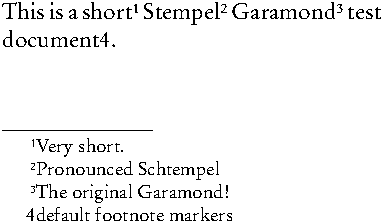
\includegraphics{stempelfoot0-crop} \qquad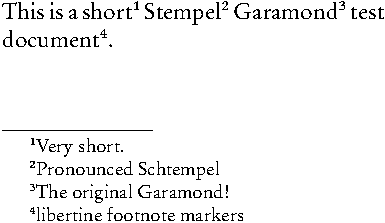
\includegraphics{stempelfoot1-crop}\]
%This package redefines these macros so that \verb|\sustyle| changes the font and applies the scaling changes, while changes due to the {\tt raised} parameter are applied only within \verb|\textsu|. For this reason, we have to modify the definition of \verb|\@makefnmark| as essentially as follows, when not in a minipage:
%\begin{verbatim}
%\def\@makefnmark{\raisebox{\superiors@raised}{\hbox%
%        {\sustyle\hspace*{\superiors@spaced}\@thefnmark%
%        \hspace*{.03em}}}}
%\end{verbatim}
%
%Relatively few Opentype text font families have a complete set of superior figures that can be accessed after running \textsf{otfinst}. 
The following have a complete set of superior figures:
\begin{verbatim}
newtxtext
newpxtext
libertine
libertinus-serif
TeXGyreTermesX
TeXGyrePagellaX
Erewhon
Heuristica
Baskervaldx
EBGaramond
garamondx
XCharter
baskervillef
cochineal
STIX2
stickstoo
fbb
ETbb
Adobe Bembo Std
Adobe Caslon Pro
Adobe Warnock Pro
Monotype Dante Std
Monotype Bell Std
Monotype Perpetua Std
Adobe Garamond Premier Pro
Adobe Brioso Pro
Adobe Arno Pro
Adobe Kinesis Std
Adobe Jenson Pro
Adobe Kepler Std
\end{verbatim}
(Those listed without a vendor name are free, and mostly available through \TeX Live.)

A second problem is the current paucity of fonts containing a full set of superior symbols that may be required. Note that {\tt latex} does a good job using faked superiors, but they don't always have the quality of real superiors. Currently (January 2024), from the list above, only the first two provide superior versions of these symbols. Even if the opentype font contains them and they are correctly referenced in the {\tt sups} lookup table so that they function properly with {\tt lualatex} and {\tt xelatex}, legacy latex may fail because the latex font family for superiors does have a TS1 fd file by which to locate them. This is the case with {\tt EBGaramond}, for example.

The next four pages show some footnote examples, all made with {\tt lualatex} and {\tt superiors} but with either {\tt article} or {\tt scrartcl} and either {\tt newtxtext} or {\tt newpxtext}.
\newpage
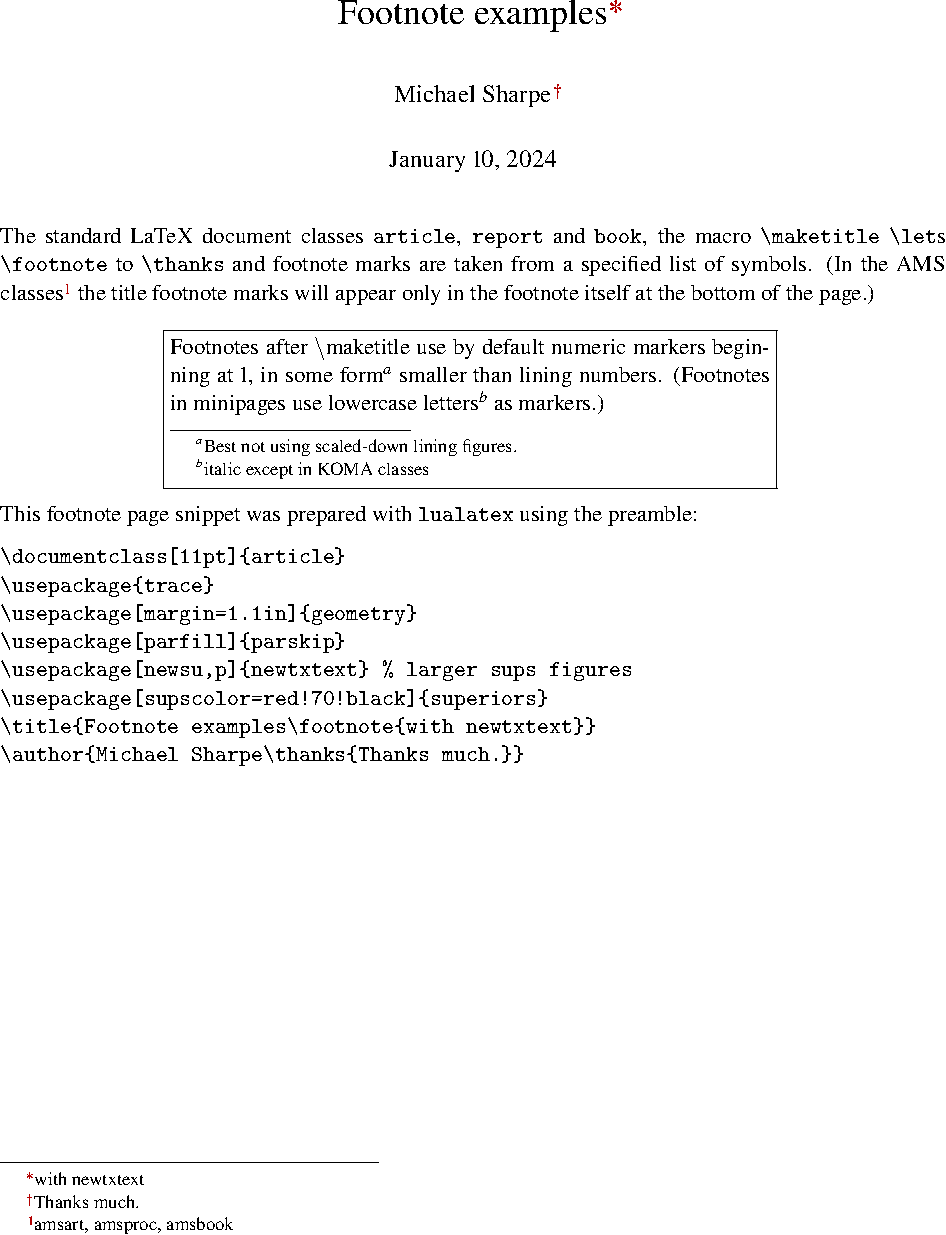
\includegraphics{footsnippet1-crop.pdf}
\newpage
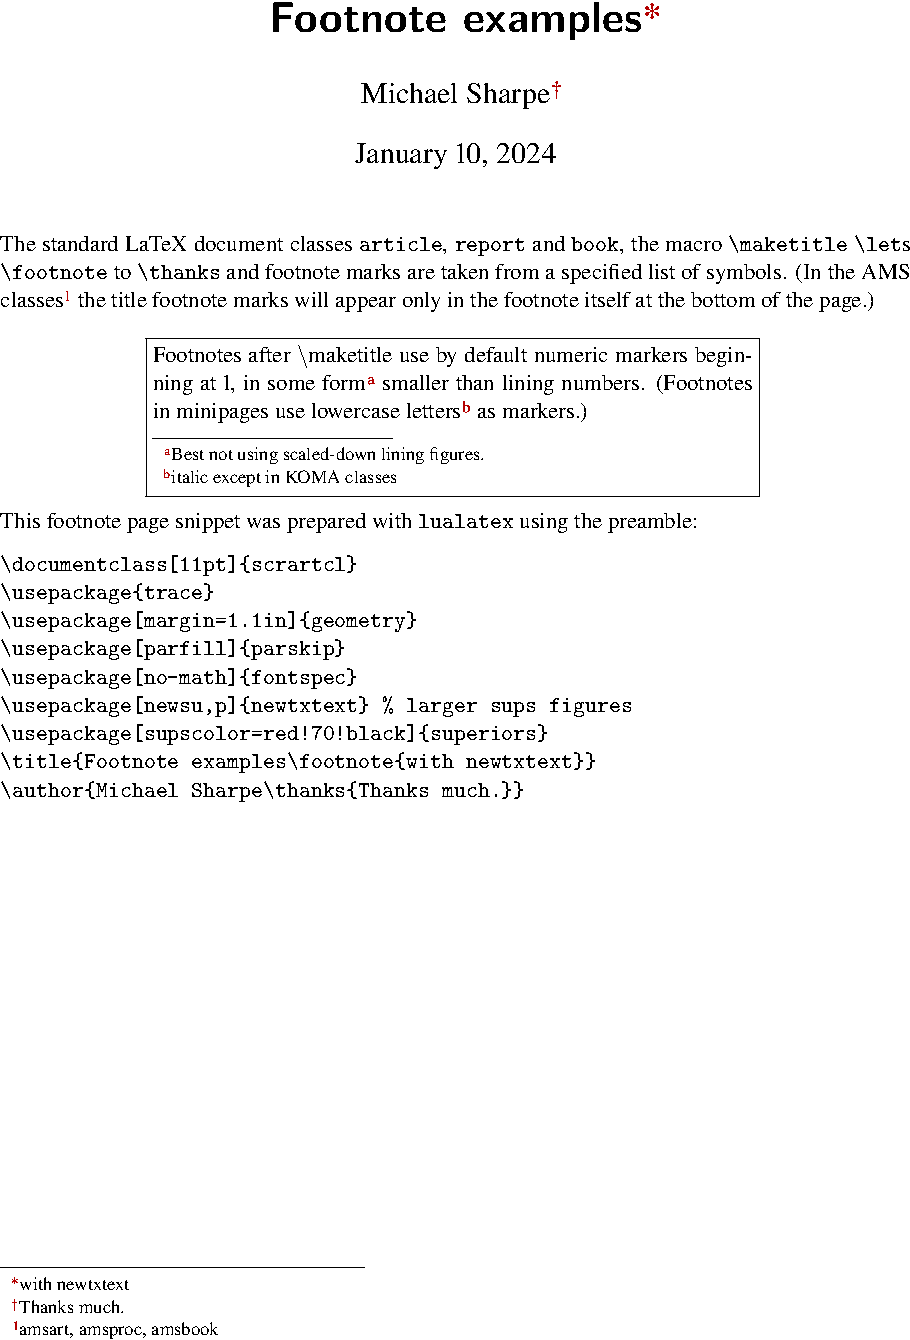
\includegraphics{footsnippet2-crop}
\newpage
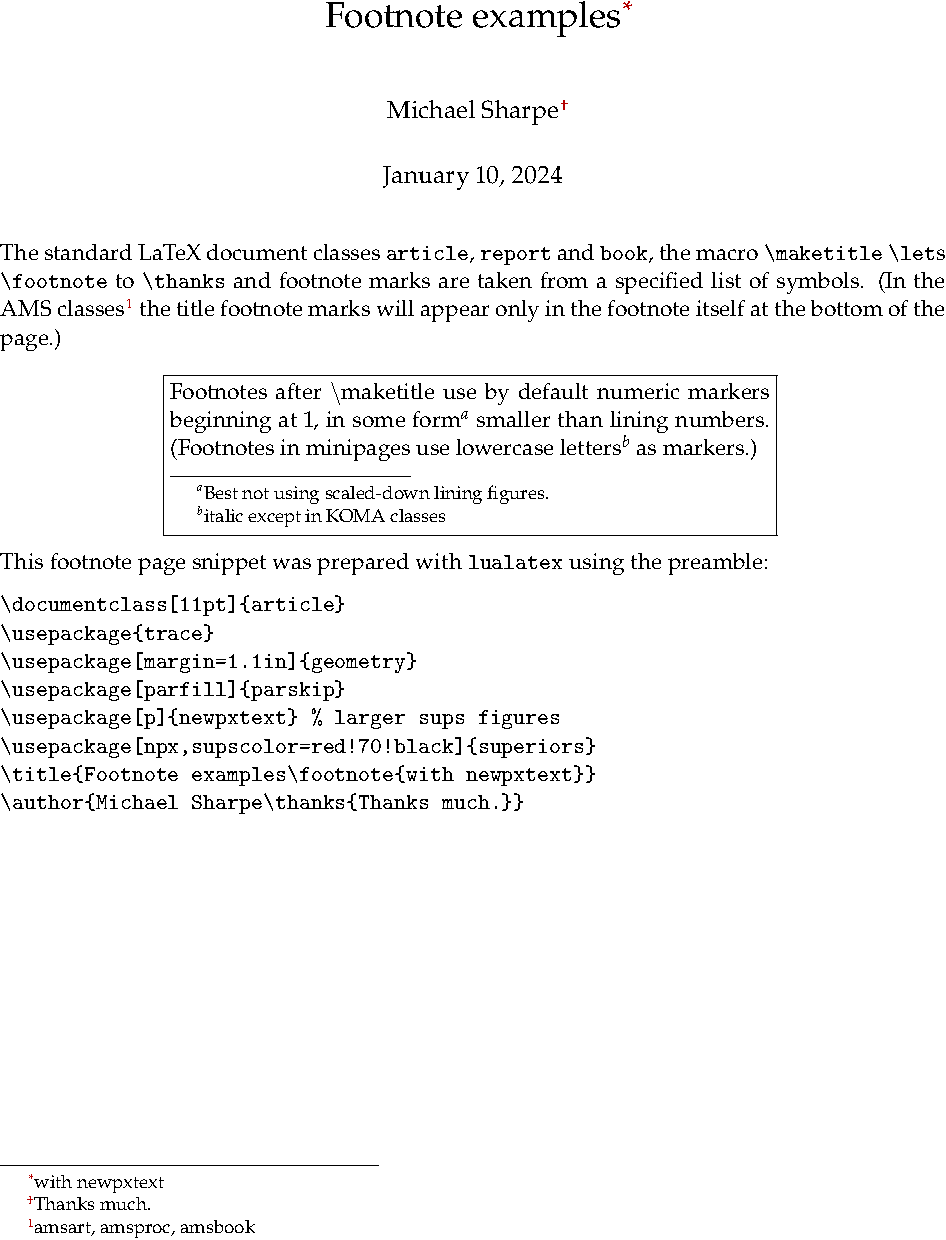
\includegraphics{footsnippet3-crop}
\newpage
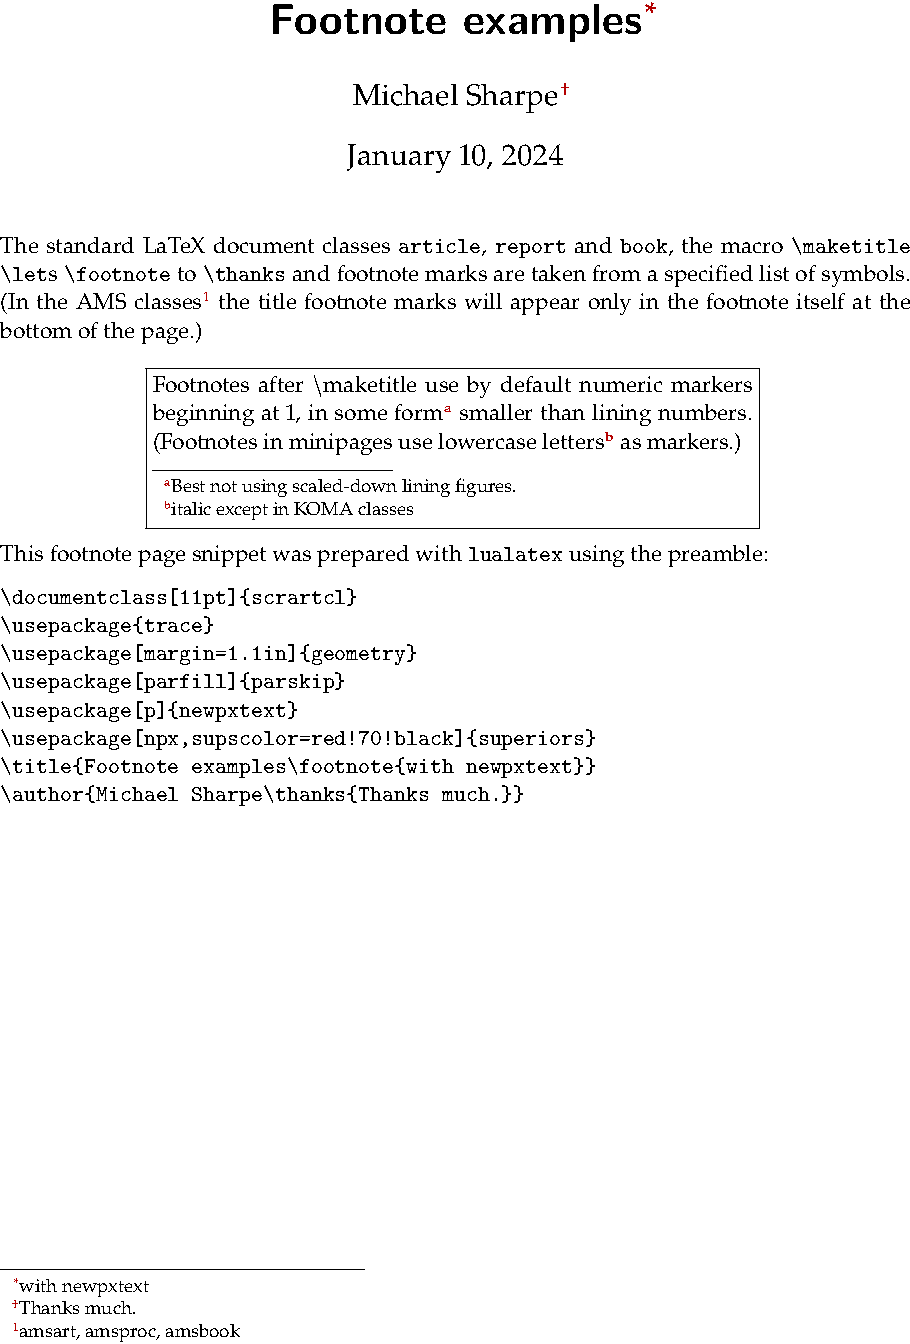
\includegraphics{footsnippet4-crop}
\end{document}  